\chapter{Determining the presence of NLOS component}

The first set of practical measurements was carried out in order to determine the presence and observe the characteristics of the non-line-of-sight component of the signal. 

\section{Measurements setup}

The measurements were obtained using Nokia's sensing proof-of-concept described in section \ref{sec:intro-PoCarchitecture}. The system was mounted in an indoor scenario, with the receiver positioned at a height of $5,12$ m. The transmitter was positioned towards an open indoor area, located approximately 23 metres away from a warehouse rack (which was in front of a wall) and a cargo door.
The objective was to obtain a non-line-of-sight measurement by reflecting the signal on the wall and subsequently on a moving target. 

The tests were carried out using:

\begin{enumerate}
	\item A human target.
	\item A strong reflector (large metal cabinet with flat surfaces).
\end{enumerate}

The direction (azimuth $\theta$ and elevation $\varphi$) of the transmitted beam was fixed for the whole measurement.

Before each test, a short calibration measure is performed, which includes only the static elements of the scenario. The calibration data will be used in the post-processing steps for subspace-based clutter removal with the CRAP method  \cite{Henninger_Mandelli_Grudnitsky_Wild_Brink_2023}. 

\section{Moving target without obstructions}

The OFDM radar system will be able to determine the range and radial speed component (the angle of arrival AOA is fixed). During the initial measurement the antenna boresight was directed perpendicular to the wall,while the target moved radially between the transmitter and reflector.

Beam elevation was chosen to be as high as possible in order to avoid line-of-sight from the transmitted beam's main lobe. Beam parameters are shown in table \ref{table:Test1TXBeamParams}.


% TODO: substitute placeholder table
\begin{table}[H]
	%\caption*{\textbf{Title of Table (optional)}}
	\centering 
	\begin{tabular}{|p{9em} c c c |}
		\hline
		\rowcolor{bluepoli!40} % comment this line to remove the color
		\textbf{Substitute placeholder table} & \textbf{} & \textbf{} & \textbf{Time aperture [ms]} \T\B \\
		\hline \hline
		$\textbf{Standard frame}$ & 60,91 & 1120 & 10 \T\B \\
		$\textbf{Decimated frame}$ & 45,16 & 24 & 10 \T\B\\
		$\textbf{6 frames}$ & 52,35 & 96 & 60  \T\B\\
		$\textbf{10 frames}$ & 54,66 & 160 & 100  \T\B\\
		
		\hline
	\end{tabular}
	\\[10pt]
	\caption{Transmitted beam parameters for initial measurements.}
	\label{table:Test1TXBeamParams}
\end{table}

Since only the radial component of speed can be measured, the aim of the test was to maximize this component in order to analyze the characteristics of the signal generated from the reflection.

\subsection{Line-of-sight and non-line-of-sight separation}

In addition to clutter removal, calibration measurements provide valuable information for the determination of the distance threshold at which targets can be accurately classified as NLOS. To this end, certain calibration frames can be processed as radar frames, focusing on the analysis of the zero-doppler component.
	
	
% TODO: cambiare figura, metterne una con solo il muro
\begin{figure}
	\centering
	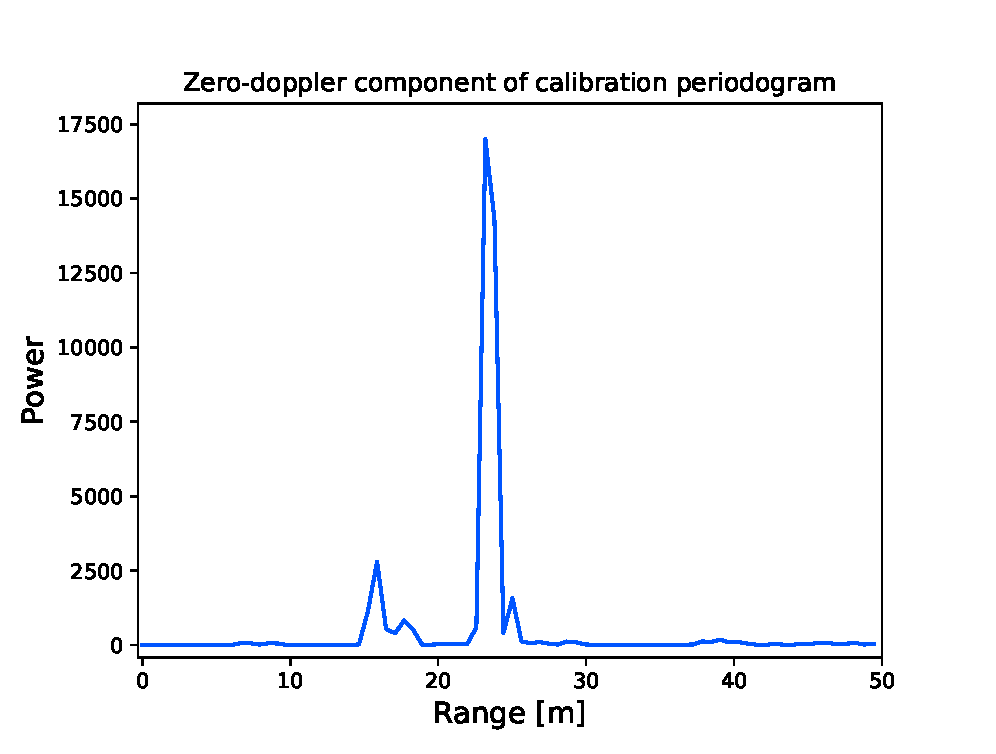
\includegraphics[width=0.6\textwidth]{Images/To-be-sorted/cali_static_per/cali_static_per.eps}
	\caption{Zero doppler component of a periodogram generated from calibration measurements}
	\label{fig:Test1_cali_static_per}
\end{figure}

As can be seen in the figure \ref{fig:Test1_cali_static_per}, a large target is present approximately $23$ m from the system. It was assumed that any target return associated with a range greater than $23$ m was generated by a signal reflected from the main target.

After the periodogram has been generated, this separation can be taken into account in the post-processing phase to process the NLOS section separately from the LOS section.



